\documentclass{beamer}
\usepackage{tabularx}
\mode<presentation>
{
  %\usetheme{Warsaw}
  % or ...
  \usecolortheme{beaver}

  \setbeamercovered{transparent}
  % or whatever (possibly just delete it)
}

\title{ADPLL Network on an FPGA}
\author{Conor Dooley}
\subtitle{Semester 1 Presentation}

\begin{document}

\begin{frame}
    \titlepage
\end{frame}

\section*{Background/Literature Review}
\begin{frame}{Motivation}
  % - A title should summarize the slide in an understandable fashion
  %   for anyone how does not follow everything on the slide itself.
	\begin{itemize}
        \item[--]
            \textbf{Reminder:} A Phase Lock Loop outputs a signal phase synchronised with a multiple of the reference.
            \begin{center}
            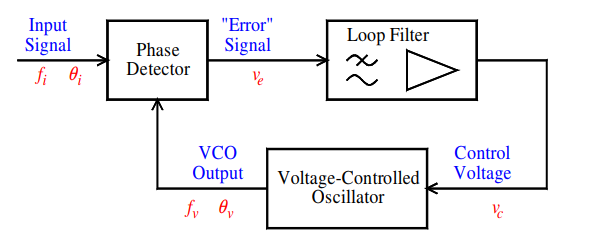
\includegraphics[scale=0.3]{mulkeen_pll}
            \begin{tiny}\begin{flushright}\cite{bm_slides}\end{flushright}\end{tiny}
            \end{center}
        \item[--]
            ADPLL - All Digital PLL:
            \begin{itemize}
	        \item[]
	            Number controller oscillator $\rightarrow$ quantised frequency.
	        \item[]
	            Digital phase detector output $\rightarrow$ quantised phase difference.
        	\end{itemize}
        \end{itemize}
    \begin{itemize}
        \item[--]
        	Want low power, high frequency clocking system for SoCs.
        \item[--]
            Want closely sync'ed clocks, characterised using:
    		\begin{itemize}
    			\item[]
    				Average difference \textit{skew}.
    			\item[]
	    			Gaussian random process \textit{jitter}.
    		\end{itemize}
    \end{itemize}
\end{frame}

\begin{frame}{Existing Solutions}
  % - A title should summarize the slide in an understandable fashion
  %   for anyone how does not follow everything on the slide itself.
	\begin{columns}
		\column{0.55\linewidth}
		\textbf{Branch, H, X trees}
		\begin{itemize}
			\item[--]
				Use buffers \& delay symmetry.
			\item[--]
				Fabrication mismatch problems $\rightarrow$ skew, high power usage.
		\end{itemize}
		\textbf{Clock Mesh}
		\begin{itemize}
			\item[--]
				Great timing accuracy.
			\item[--]
				Redundancy $\rightarrow$ very high power draw.
		\end{itemize}
		\textbf{Skew Compensation}
        \begin{itemize}
        	\item[--]
        		Centralised/Decentralised methods.
	        \item[--]
	            Increases power consumption.
	    \end{itemize}
		\column{0.45\linewidth}
			%\centering	
			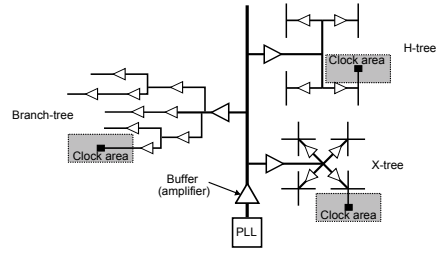
\includegraphics[scale=0.4]{eldar_trees}
			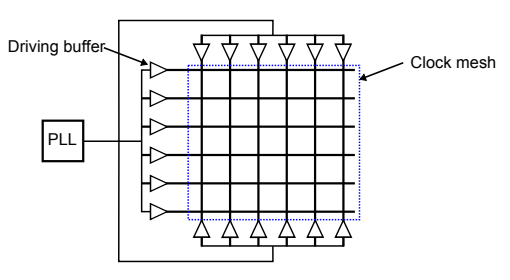
\includegraphics[scale=0.4]{eldar_mesh}
			\begin{tiny}\begin{flushright}\cite{eldar}\end{flushright}\end{tiny}
	\end{columns}
 
\end{frame}

\begin{frame}{ADPLL Network}
        
        \begin{columns}        	
        	\column{0.65\linewidth}
        	\textbf{PLL network:}
	        \begin{itemize}
			    \item[]
			       	PLLs generate clock in an area of chip.
			    \item[]
			        Synced via lower freq. error signal between neighbouring PLLs.
    		\end{itemize}
        	\column{0.35\linewidth}
        	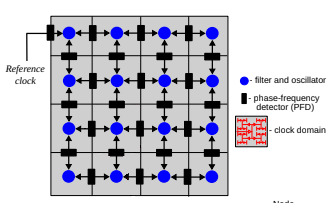
\includegraphics[scale=0.55]{network_ccic2013}
        	\begin{tiny}\begin{flushright}\cite{eldar}\end{flushright}\end{tiny}
        \end{columns}
        \begin{columns}
            \column{\linewidth}
            \vspace{0.1 cm}
    	    \textbf{Example node:}
    	    \begin{center}
		    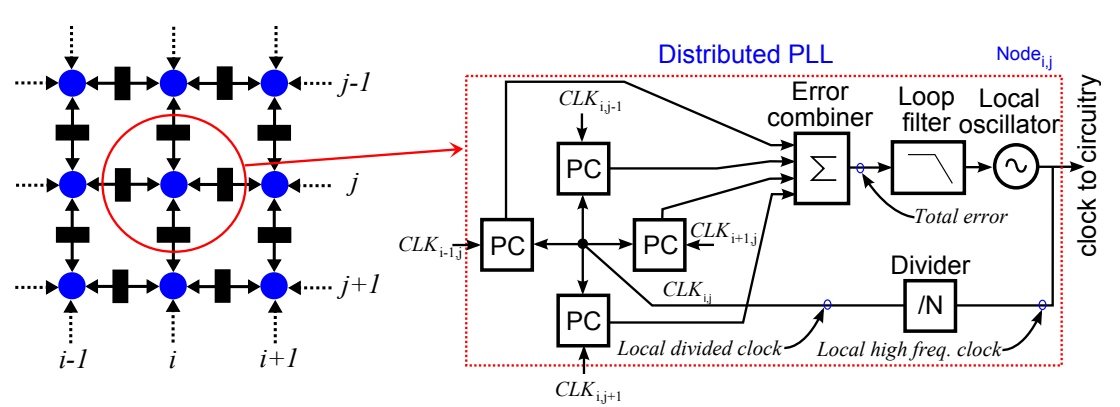
\includegraphics[scale=0.3]{eldar_node}
		    \end{center}
		    \begin{tiny}\begin{flushright}\cite{eldar}\end{flushright}\end{tiny}
        \end{columns}
\end{frame}

\iffalse
\section*{ADPLL Network}
\begin{frame}{ADPLL Network on an FPGA}
  % - A title should summarize the slide in an understandable fashion
  %   for anyone how does not follow everything on the slide itself.

    \begin{itemize}
        \item[--]
            An FPGA is the optimum platform for rapid physical prototyping \& enables limited validation.
        \item[--]
        	Enables low cost testing of potential network architectures and control schemes.
        	%TODO ask Elena for a good thing to say here
        \item[--]
        	FPGA implementation brings with it some challenges:
        	\begin{itemize}
        		\item[]
        			Restriction placed on available hardware. No gates, only LUTs.
        		\item[]
        			No delay lines for time-digital converter.
        		\item[]
        			Frequency must be downscaled to MHz from GHz region.
        		\item[] 
        			Synchroniser to avoid metastability in phase detector sets phase difference step size.
        			%TODO any more?        		
        	\end{itemize}
    \end{itemize}
%The aim of this project is to investigate alternative methods of implementing an ADPLL on an FPGA, and ultimately to build a network of ADPLLs on an FPGA, along with hardware to allow its performance to be measured. This will allow the real-world behaviour of such a system to be analysed, and compared with existing simulation models. It will allow new architectures to be tested, and act as a step on the path to an IC prototype. 
\end{frame}
\fi %TODO keep this? @mulkeen

\begin{frame}{My ADPLL}
  % - A title should summarize the slide in an understandable fashion
  %   for anyone how does not follow everything on the slide itself.
 	%\begin{columns}
 	\begin{center}
 		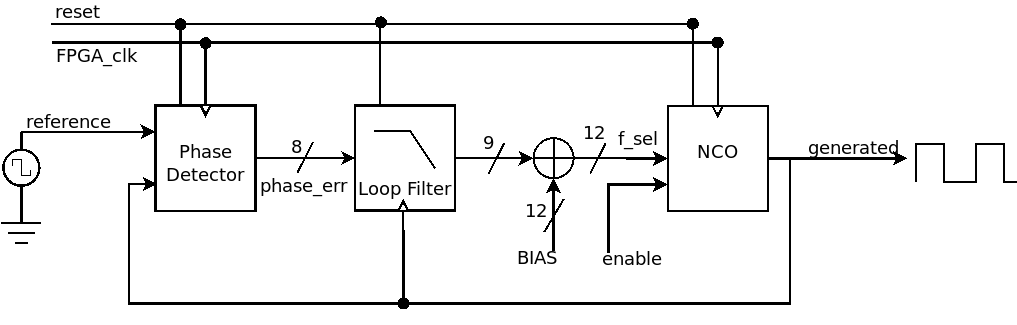
\includegraphics[scale=0.25]{../rtl}
 	\end{center}
		
	\begin{itemize}
		\item[--]
			2 different oscillators made - Inverter Chain \& Phase Accumulator.
		\item[--]
            12 bit Phase Accum. used, 9 LSB control code, $62.988\textrm{ kHz}$  frequency step.
		\item[--]
			5 MHz bias point, FPGA clock at 258 MHz.		
		\item[--]
			8 bit Phase Detector, resolution of $6.975^\circ$ at 5 MHz.
		\item[--]
			9 bit PI Loop Filter. %from paper as a viable value
	\end{itemize}
	%\end{columns}
\end{frame}

\begin{frame}{Phase Detector}
  % - A title should summarize the slide in an understandable fashion
  %   for anyone how does not follow everything on the slide itself.
    \vspace{-0.67 cm}
    \begin{center}
        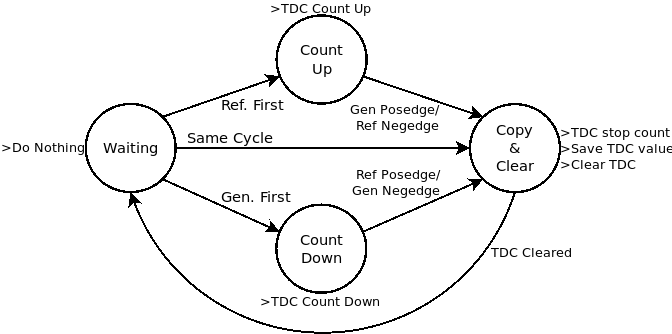
\includegraphics[scale=0.35]{../state_trans_diagram.png}
 	\end{center}
    \vspace{-0.1 cm}
	\begin{itemize}
        \item[--]
            State Machine implements phase detector.
        \item[--]
            Up/Down count instruction sent to 8 bit TDC.
        \item[--]
            Save/Clear overwrites previous output.
        \item[--]
            Negedge condition avoids potential signal miss.
    \end{itemize}
	%\end{columns}
\end{frame}

\begin{frame}{Loop Filter}
  % - A title should summarize the slide in an understandable fashion
  %   for anyone how does not follow everything on the slide itself.
    \vspace{-0.67 cm}
 	\begin{center}
        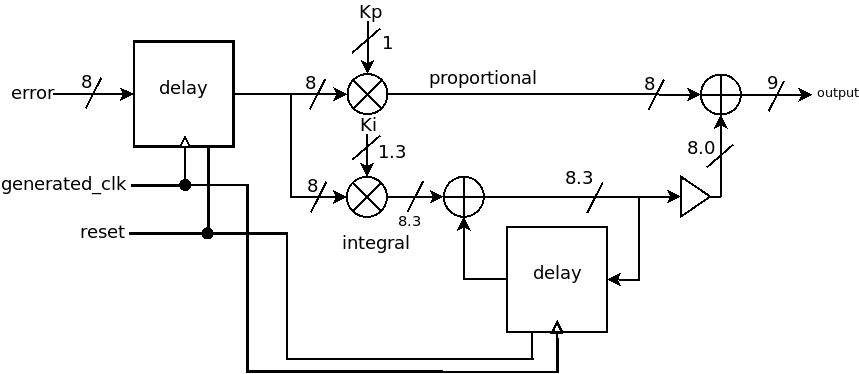
\includegraphics[scale=0.325]{../loop_filter.png}
 	\end{center}	
	\begin{itemize}
		\item[--]
            Loop Filter implemented by a PI controller.
        \item[--]
            Coefficients of $k_p=1$ \& $k_i=0.125$ chosen for stability. \cite{pid_coeffs}
        \item[--]
        	8 bits signed input, 9 bits signed output.
        \item[--]
        	Output + bias = control code
    \end{itemize}
	%\end{columns}
\end{frame}

\begin{frame}{Number Controller Oscillators}
  % - A title should summarize the slide in an understandable fashion
  %   for anyone how does not follow everything on the slide itself.	
	\begin{itemize}
		\item[--]
            Inverter Ring \& Phase Accumulator
        \item[--]
            Ring harder to implement, but more realistic.
        \item[--]
            $0.63\textrm{ ns}$ per inverter, currently 4 control bits.
        \item[--]
        	Phase Accum. relies on FPGA clock \& bias.
        \item[--]
        	12 bit Phase Accumulator, 9 LSB control code, $62.988\textrm{ kHz}$ frequency step.
    \end{itemize}
	%\end{columns}
\end{frame}

\section*{Measurements}
\begin{frame}{Simulations}
% - A title should summarize the slide in an understandable fashion
%   for anyone how does not follow everything on the slide itself.
	\vspace*{-10mm}
 	\begin{center}
 		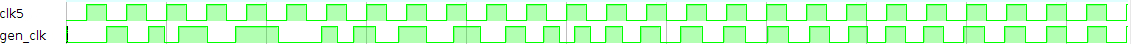
\includegraphics[scale=0.25]{../vivado_sim}
 	\end{center}
	\begin{columns}
	\column{0.5\linewidth}
    \begin{itemize}
	    \item[--]
	        Simulated in Vivado to verify behaviour.
	    \item[--]
	        Individually tested blocks using simulation.
	    \item[--]
	        Simulated locking to a reference signal.
	    \item[--]
            Observed jitter of $3.491$ ns, predicted p2p of $21.579\textrm{ ns}$.
	    \item[--]
            $20.91\textrm{ }\mu\textrm{s}$ to lock, initial deviation of $213\textrm{ kHz}$.
	\end{itemize}
	
    \column{0.5\linewidth}
	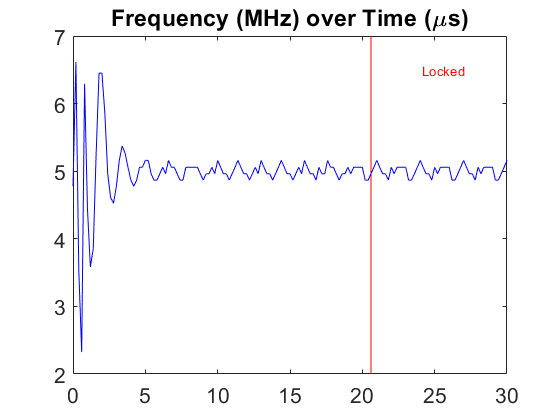
\includegraphics[scale=0.4]{../sim_locking}
	\end{columns}

\end{frame}

\begin{frame}{Measurements}
  % - A title should summarize the slide in an understandable fashion
  %   for anyone how does not follow everything on the slide itself.
	\vspace*{-5mm}
	\begin{center}
		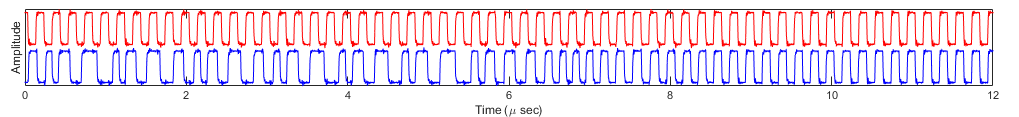
\includegraphics[scale=0.425]{../impl_waveform}
	\end{center}
   	\begin{columns}
    	\column{0.5\linewidth}
    	\begin{itemize}
            \item[--]
                Tested with $f_c=5.04\textrm{ MHz}$, ($\textrm{BIAS}=80$).
    		\item[--]
	    		Lock range: $4.19\rightarrow12.34\textrm{ MHz}$ 
            \item[--]
                Capture range: $4.25\rightarrow12.76\textrm{ MHz}$
            \item[--]
                Free running jitter: $200.1665\pm1.9689\textrm{ ns}$.
            \item[--]
                Locked jitter: $200.009\pm2.7378\textrm{ ns}$
            \item[--]
                $24.6\textrm{ }\mu\textrm{s}$ to lock, initial deviation of $213\textrm{ kHz}$. 
        \end{itemize}
    	
        \column{0.5\linewidth}
    	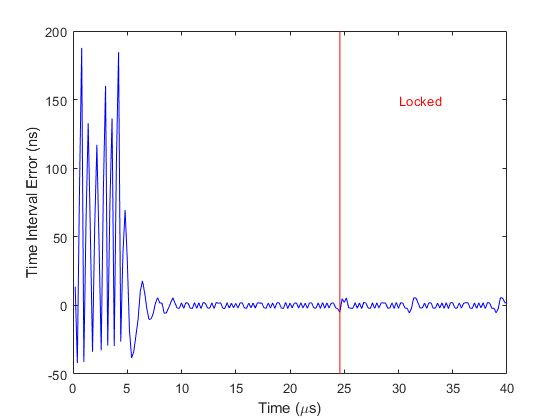
\includegraphics[scale=0.4]{../impl_locking}
    \end{columns}
\end{frame}

\begin{frame}{Measurement Difficulties}
% - A title should summarize the slide in an understandable fashion
%   for anyone how does not follow everything on the slide itself.
\vspace*{-5mm}
%\begin{center}
%	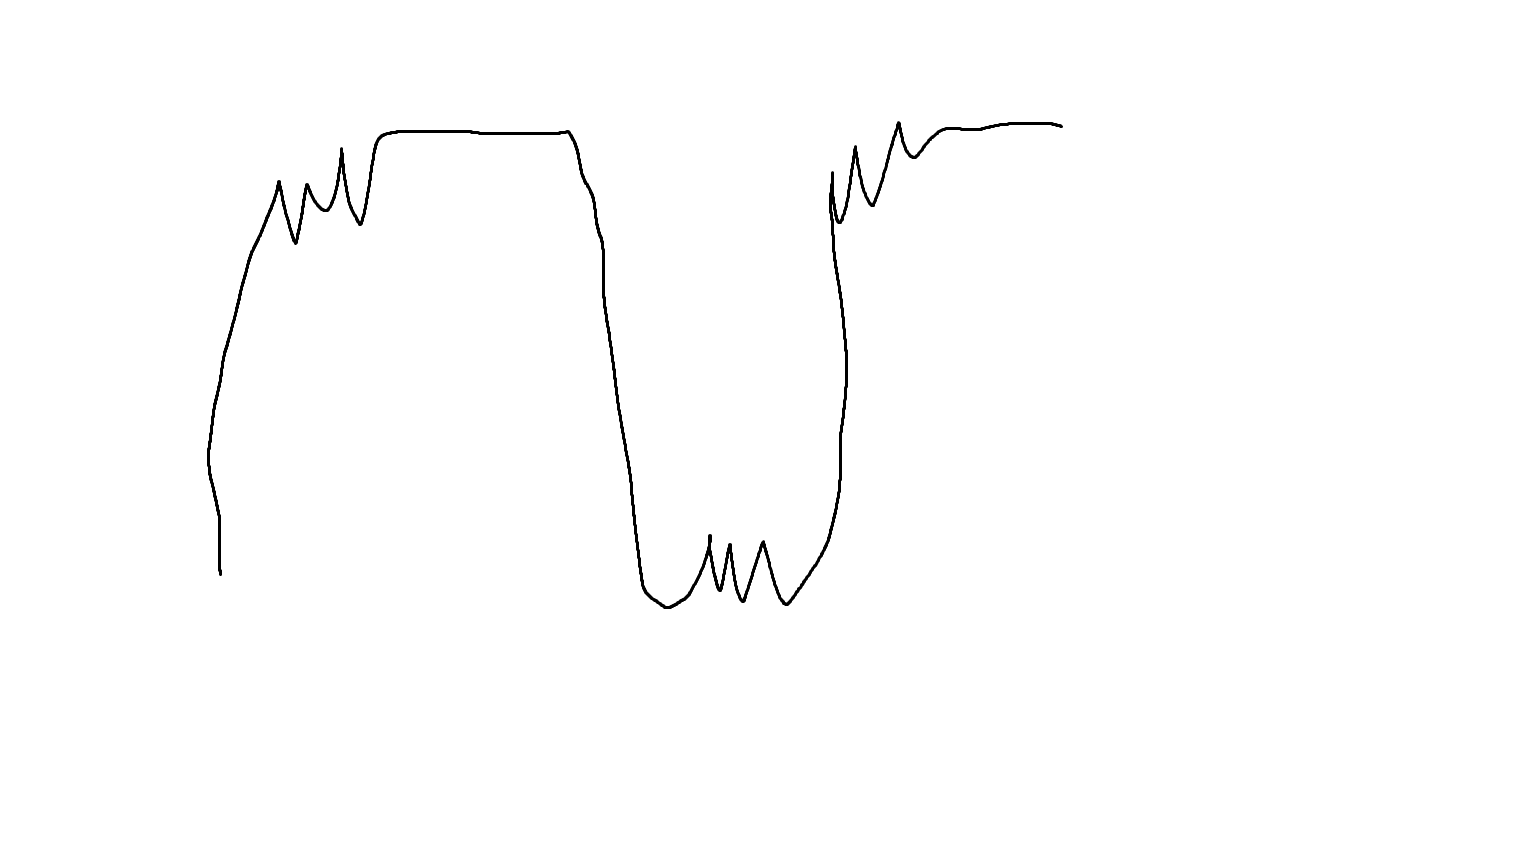
\includegraphics[scale=0.1]{../bad_waveform}
%\end{center}
\begin{columns}
	\column{0.5\linewidth}
	\begin{itemize}
		\item[--]
			FPGA doesn't have a suitable RF (in/out)put.
		\item[--]
			Using jumper wires currently.
		\item[--]
			Resulting waveforms show some distortion.
		\item[--]
			$f_c>>5\textrm{ MHz}$ leads to significant distortion.
	\end{itemize}
	\column{0.5\linewidth}
    \includegraphics[angle=270,origin=c,scale=0.04]{../measurement_setup.jpg}

\end{columns}
\end{frame}

\section*{Future Work}

\begin{frame}{Future Work}
  % - A title should summarize the slide in an understandable fashion
  %   for anyone how does not follow everything on the slide itself.
%TODO dates
    \begin{itemize}
        \item[1]
            Implement external reference. %\date{Before end of week.}
        \item[2]
            Create PLL using Inverter Chain. %\date{Before end of exams}
        \item[3]
            Small scale interlinked PLLs. %\date{???}
        \item[4]
            Acquire more suitable FPGA for measurements. %\date{Before end of study week}
        \item[5]
            Build small scale network. % \date{Jan}
        \item[6]
            Test said network on FPGA. % \date{Jan}
        \item[7]
            Perform more thorough analysis of results. % \date{?}
    \end{itemize}
 
\end{frame}

\begin{frame}{Reference}
  %\frametitle<presentation>{For Further Reading}
	\begin{columns}
		\column{0.6\linewidth}
		\begin{thebibliography}{10}
		\begin{tiny}
		\setbeamertemplate{bibliography item}{}
		% Followed by interesting articles. Keep the list short.
		\bibitem{read_first}
		M. Javidan, et al.
		\newblock All-digital PLL array provides reliable distributed clock for SOCs.
		\newblock {\em IEEE International Symposium on Circuits and Systems}, 2589-2592, 2011. %PID coefficients	
  	
	  	% Start with overview books.
	  	\bibitem{eldar}
	    E. Zianbetov.
	    \newblock {\em Distributed Clocking For Synchronous SoC}.
		\newblock Universit\'e Pierre et Marie Curie, 2013. %network architecture
		
		\bibitem{shan}
		C. Shan.
		\newblock {\em Distributed Clocking For Synchronous SoC}.
		\newblock Universit\'e Pierre et Marie Curie, 2014. %network architecture
		
	 	 % Followed by interesting articles. Keep the list short.
	  	\bibitem{pid_coeffs}
	    E. Koskin, et al.
	    \newblock Generation of a Clocking Signal in Synchronized All-Digital PLL Networks.
	    \newblock {\em IEEE Transactions on Circuits and Systems II: Express Briefs}, 65(6), 809-813, 2018. %PID coefficients

	    \bibitem{bm_slides}
	    B. Mulkeen.
	    \newblock Wireless System Notes, .
	    \newblock {\em IEEE Transactions on Circuits and Systems II: Express Briefs}, 65(6), 809-813, 2018. %PID 
	    
	    %\bibitem{network_ccic2013}
	    %E. Zianbetov, et al.
	    %\newblock {\em Distributed clock generator for synchronous SoC using ADPLL network}.
	    %\newblock {\em Custom Integrated Circuits Conference (CICC)}, IEEE, 2013. %images
	    \end{tiny}
	  	\end{thebibliography}
  		\column{0.4\linewidth}
  		\begin{itemize}
  			\item[$\rightarrow$] Background Info
  			\vspace{0.6 cm}
  			\item[$\rightarrow$] ADPLL/DCO Design
  			\vspace{0.6 cm}
  			\item[$\rightarrow$] ADPLL Network
  			\vspace{0.6 cm}
  			\item[$\rightarrow$] Filter Coefficients
  		\end{itemize}
  \end{columns}
\end{frame}

\section*{Summary}

\begin{frame}{Summary}

  % Keep the summary *very short*.
    \begin{itemize}
        \item[--]
            FPGA based analysis platform for ADPLL network designs.
        \item[--]
            Designed and implemented a single ADPLL.
        \item[--]
            Simulated and performed basic measurements on ADPLL.
    \end{itemize}

  % The following outlook is optional.
    \vskip0pt plus.5fill
    \begin{itemize}
        \item[--]
        Near Future:
        \begin{itemize}
            \item[]
                %Brief outlook
                External reference \& inverter chain ADPLL.
            \item[]
                Source higher performance FPGA.
    \end{itemize}
  \end{itemize}
\end{frame}

\end{document}
